\documentclass{beamer}
\usetheme{CWRU}

\title{Exploring Alternative Routes Using Multipath TCP}
\author{Stephen Brennan}
\institute{Case Western Reserve University}
\date{June 5, 2017}

\usepackage{appendixnumberbeamer}
\usepackage{pgfpages}
\usepackage{wrapfig}
\usepackage[export]{adjustbox}
\usepackage{graphicx}
\usepackage{fancyvrb}
\usepackage{bytefield}
\usepackage[style=authoryear,backend=bibtex]{biblatex}
\setbeamertemplate{note page}[plain]
\setbeameroption{show notes on second screen=right}
\setbeamertemplate{navigation symbols}{}%remove navigation symbols
\AtBeginNote{%
    \let\enumerate\itemize%
    \let\endenumerate\enditemize%
}

\bibliography{paper}

\newcommand{\FigureSlide}[2]{
  \begin{frame}[plain]
    \begin{centering}
      \vfill
      \includegraphics[max width=\textwidth,max height=\textheight]{#1}
      \vfill
      \end{centering}
    \note{#2}
  \end{frame}
}

\newcommand{\TitledFigureSlide}[3]{
  \begin{frame}{#2}
    \begin{centering}
      \vfill
      \includegraphics[max width=\textwidth,max height=\textheight]{#1}
      \vfill
      \end{centering}
      \note{#3}
  \end{frame}
}

\newcommand{\SectionHead}[2]{
  \begin{frame}{#1}
    \tableofcontents[currentsection,hideallsubsections]
    \note{#2}
  \end{frame}
}

% fuckit
\newcommand{\mycitetext}[1]{
  \citeauthor{#1}. \citetitle{#1}. \citeyear{#1}
}
\newcommand{\mycite}[1]{
  \footnote{\mycitetext{#1}}
}

\begin{document}
\frame{
  \titlepage
  \note{
    Hello everyone. I'm Stephen, and today I'll be discussing my thesis,
    entitled ``Exploring Alternative Routes Using Multipath TCP''.
  }
}

\section{Introduction}

\begin{frame}{Overview}
  \tableofcontents[hideallsubsections]
  \note{

    \textbf{Transition:} Here is an overview of how this talk is organized.

    \begin{itemize}
    \item Start with an Introduction motivating this thesis, ending with a
      problem statement
    \item Background on Multipath TCP
    \item Related work such as overlays
    \item Implementation of the project
    \item Experimental evaluation
    \item Conclude with discussion of related work and a summary
    \end{itemize}

  }
\end{frame}

\TitledFigureSlide{figures/InternetSlide.pdf}{Internet Architecture}{

  \textbf{Transition:} I would like to start this talk with a brief, simplified
  look at routing on the Internet.

  \begin{itemize}
  \item As we know, routers, ASes, in blue and tan \textbf{respectively}
  \item Routers forward packets based on routing tables
  \item Tables built via ``distributed shortest path algorithms'', optimal in
    terms of AS-hops
  \item Inefficiencies result for particular paths
    \begin{itemize}
    \item AS hops doesn't take into account path bandwidth, congestion, etc
    \item ASes are businesses, make policies and route based on financial bottom
      line
    \end{itemize}
  \end{itemize}

}

\begin{frame}
  \frametitle{Internet Routing Inefficiencies}
  \begin{columns}
  \begin{column}{0.7\textwidth}
  \begin{itemize}
  \item The default route is not always the best, in terms of latency or
    reliability
  \item Peering agreements and policy based routing can result in suboptimal
    routing decisions \footnotemark
  \item A route that passes through a ``detour'' may be better
  \end{itemize}
  \end{column}
  \begin{column}{0.3\textwidth}
    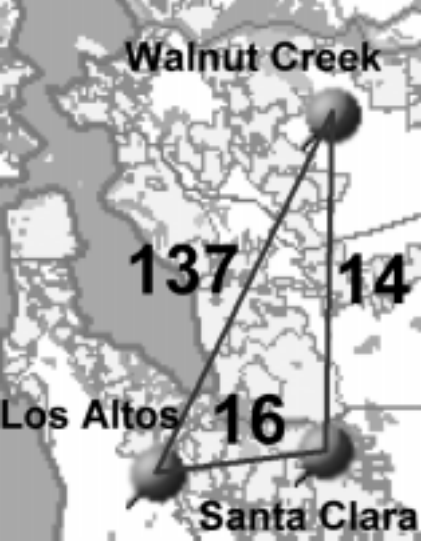
\includegraphics[width=\textwidth]{figures/detour.png} \\
    \textit{Example of an inefficient default route \footnotemark[1]}
  \end{column}
  \end{columns}
  \footnotetext{\mycitetext{detour}}
  \note{

    \begin{itemize}
    \item Not simply something we can hypothesize about.
    \item Real world examples show that default routes aren't the best paths for
      users.
    \item In fact, many times you can add a ``detour'' to your route and end
      up with an improved path.
    \item At right, the default path from Los Altos to Walnut Creek has round
      trip time of 137 milliseconds, while the constituent paths of a detour
      route through Santa Clara add up to 30 milliseconds
    \end{itemize}

  }
\end{frame}

\FigureSlide{figures/detour-packetloss.png}{

  \begin{itemize}
  \item Not just isolated examples.
  \item Same study looked at a group of computers across universities
  \item Observed pairwise RTT, loss rate.
  \item Searched for pairs where ``triangle inequality violated'', i.e. lower
    RTT or loss rate via detour.
  \item In graph, blue is default route, yellow is best alternative route, and
    we compare loss rate
  \item For 80\% of pairs, alternative route is more reliable. For 25\% of
    pairs, alternative route improves loss rate by at least a factor of 6
  \item For some pairs, reliability difference is staggering!
  \end{itemize}

}

\begin{frame}
  \frametitle{Access Link Underutilization}
  \begin{itemize}
  \item Residential bandwidth constantly improves
  \item However, residential bandwidth is not fully utilized
    \mycite{fibertothehome}
    \begin{itemize}
    \item Short-lived TCP sessions?
    \item Anemic send buffers?
    \item Network core can't support bandwidth?
    \end{itemize}
  \item Using alternative routes can improve performance
  \item Aggregating multiple routes can perform even better
  \end{itemize}

  \note{

    \textbf{Transition:} Take a brief detour and discuss residential access
    speeds. (lol detour)

    \begin{itemize}
    \item Residential access links always increasing
    \item Dial-up, broadband, cable, now fiber-to-the-home
    \item Local study on fiber connections shows bandwidth not fully utilized
      (go over each possibility, incl send buffer ``anemia'')
    \item If network core can't support bandwidth, the detour routing approach
      can help
    \item If we have plenty of access bandwidth, why not aggregate paths we have
      available to us?
    \end{itemize}

  }
\end{frame}

\TitledFigureSlide{figures/Concept.pdf}{Concept}{
  \begin{itemize}
  \item Detour routing has shown promise for a long time
  \item Some applications have been able to leverage it (e.g. Bittorrent)
  \item However, few unmodified applications may use the detour routing strategy
  \item Our concept is to use MPTCP to achieve detour routing in unmodified
    applications
  \item We use tunneling mechanisms to put a subflow across a detour host
  \end{itemize}
}

\begin{frame}
  \frametitle{Contributions}

  \textbf{Problem:} Unmodified applications cannot use detour routing to
  circumvent Internet routing inefficiencies.

  \vspace{0.5cm}

  \textbf{Solution:} An OS-level detour routing system that leverages Multipath
  TCP (MPTCP).

  \vspace{0.5cm}

  \textbf{Contributions:}

  \begin{itemize}
  \item A method for performing detour routing with unmodified applications
  \item A prototype implementation in the Linux kernel
  \item An evaluation of this mechanism on emulated networks and the Internet
  \end{itemize}
  \note{

    \begin{itemize}
    \item Putting together, problem: unmodified applications can't take
      advantage of detour routing solutions to Internet routing inefficiencies.
    \item A solution could be a system which uses and aggregates alternative
      routes for MPTCP connections.
    \item Contribution 1 - a mechanism for adding new routes to MPTCP
      connections which are single-homed, with no modification to applications.
    \item Contribution 2 - experimental validation that the mechanism works,
      even at higher throughputs
    \end{itemize}

  }
\end{frame}

\section{Background}
\SectionHead{}{
  \textbf{Transition:} Before explaining my solution in more detail, we'll need
  some background on Multipath TCP.
}
\subsection{Multipath TCP}

\begin{frame}
  \frametitle{Multipath TCP}

  \begin{itemize}
  \item Multi-homed devices are becoming more common
    \begin{itemize}
    \item Smartphones
    \item Datacenters
    \item Laptops
    \end{itemize}
  \item TCP still views a connection as a five-tuple: (TCP, Source IP, Source
    port, Destination IP, Destination Port)
  \item Multi-homed devices are forced to choose a network interface
  \item Multipath TCP is an extension to TCP, allowing hosts to use multiple
    addresses in the same connection
  \end{itemize}
    \note{

      \begin{itemize}
      \item Project is based on MPTCP, which enables multi-path transport for
        unmodified applications in a way not possible before
      \item Purpose is not to give complete description of MPTCP, but an
        overview
      \item Canonical motivation for MPTCP: smartphone with multiple interfaces.
      \item Also servers in datacenters (redundant topo) or laptops (wifi,
        ethernet, cell?)
      \item \textit{(See remaining slide bullets, they're good)}
      \end{itemize}

    }
\end{frame}

\begin{frame}{Design Goals}

  \begin{itemize}
  \item Remain compatible with TCP applications and the Internet
    \begin{itemize}
    \item \textit{Present the same socket API to applications}
    \item Remain similar to TCP on the wire, to remain compatible with Internet
      middleboxes
    \end{itemize}
  \item Improve performance and reliability over current TCP, by aggregating
    paths created by multiple interfaces.
  \item Do no harm to single-path TCP, by taking no more bandwidth over shared
    bottlenecks than standard TCP would
  \end{itemize}
  \note{

    \textbf{Transition:} Multipath TCP's design is motivated by several goals.

    \begin{itemize}
    \item Primary goal: compatibility
    \item Particularly API compatibility. Runs with unmodified applications
    \item Internet compat too. Middleboxes (NAT, Firewall, Normalizers, etc)
      should not be confused by, or corrupt, MPTCP
    \item Remaining two: performance, but not at the expense of existing TCP
    \end{itemize}

  }
\end{frame}

\begin{frame}[fragile]
  \frametitle{Architecture}
  \begin{center}
\begin{BVerbatim}
                     +-------------------------------+
                     |           Application         |
+---------------+    +-------------------------------+
|  Application  |    |             MPTCP             |
+---------------+    + - - - - - - - + - - - - - - - +
|      TCP      |    | Subflow (TCP) | Subflow (TCP) |
+---------------+    +-------------------------------+
|      IP       |    |       IP      |      IP       |
+---------------+    +-------------------------------+
\end{BVerbatim}
  \end{center}
  \note{

    \begin{itemize}
    \item Achieved by layering between TCP and application
    \item \textbf{Presents exact same API}
    \item \textbf{Unmodified applications can use it}
    \item Rather than creating single TCP flow, create MPTCP ``connection''
      which may contain multiple ``subflows''
    \item Subflows look very similar to regular TCP, except some TCP options
    \item Share receive window
    \item Subflows have independent sequence numbers
    \item Data has sequence numbers too
    \end{itemize}

  }
\end{frame}

\begin{frame}
  \frametitle{Path Management}

  \begin{itemize}
  \item Subflows are established with a three way handshake
  \item First subflow uses \texttt{MP\_CAPABLE} option
  \item Subsequent subflows use \texttt{MP\_JOIN} option
  \item Additional addresses may be advertised using \texttt{ADD\_ADDR} at any
    time
  \item Either side may create new subflows at any time
  \end{itemize}
  \note{

    \begin{itemize}
    \item Normal 3WHS for subflow initiation
    \item First subflow contains MP CAPABLE, exchanges key material
    \item Subsequent subflows contain MP JOIN, plus HMAC to verify identities
    \item Either side may passively announce the existence of an address
    \item Spec says nothing about when they should be created, left up to policy
    \item Kernel uses modular path manager interface for this
    \end{itemize}

  }
\end{frame}

\FigureSlide{figures/DataScheduling.pdf}{

  \textbf{Transition:} Now that we have subflows, how do we split up data across
  them?

  \begin{itemize}
  \item Again, MPTCP specifies mechanism but not policy
  \item Diagram top shows sender
  \item Data goes into scheduler, which divides it across subflows (will come
    back to that)
  \item To send it across the wire, MPTCP adds DSS option, which maps subflow
    sequence number X to data sequence number Y, for Z bytes
  \item At receiver, use options to reassemble data
  \item Data may be redundantly transferred, can't break subflow TCP semantics
  \item Scheduler has considerable freedom in dividing data
  \item Lowest RTT first ... ack-clocking
  \end{itemize}

}

\section{Related Work}
\SectionHead{}{
  \textbf{Transition:} Now in order to appreciate the place of this thesis,
  let's examine some related work. The topic includes detour routing, overlay
  routing, source routing, and multipath transport.
}

\subsection{Overlay Networks}

\begin{frame}
  \frametitle{Resilient Overlay Networks\mycite{ron}}

  \begin{itemize}
  \item Rather than use only one detour, create an overlay network
  \item Overlay nodes use the Internet as their ``link layer''
    \note[item]{In Intro, discussed Detour study. RON is something of a
      spiritual successor. Rather than simple detours, use overlay networks.}
  \item Routing performed at each node using measured link characteristics
    \note[item]{Each node is an Internet host. Constantly monitoring link
      characteristics of network, updating routing tables with performance
      metrics.}
  \item Several studies based on RON:
    \note[item]{RON achieved good results, was testbed for additional studies.}
    \begin{itemize}
    \item Redundant multipath routing\mycite{andersen2003best}
      \note[item]{One study compared two routing strategies: adaptively choosing
      the best path, or redundantly using multiple paths. No aggregation.}
  \item ``Biologically inspired'' multipath routing
    \mycite{leibnitz2006biologically}
    \note[item]{Another - biologically inspired. Choose strongest path as
      primary, have several backups, involves differential equations and
      randomness.}
  \item mTCP \mycite{zhang2004transport}
    \note[item]{mTCP: most important. A modification of TCP before
      MPTCP existed. Built on RON + userspace TCP stack. Did not have MPTCP
      compatibility concerns - routed segments across different paths. Worked on
      single-homed devices due to RON}
    \end{itemize}
  \end{itemize}

  \note[item]{\textbf{Remember:} \textit{No ``last piece'' of related work.}}
\end{frame}

\begin{frame}
  \frametitle{Other Related Items}

  \note[item]{Outside of overlay networks, several related pieces of work, both
    in research and in the standards bodies.}

  \begin{itemize}
  \item Source routing (IPv4) and segment routing (IPv6)
    \note[item]{Notable - it is possible to specify intermediaries in both IPv4
      and IPv6. For security reasons these aren't respected. Standards exist
      mainly for use in internal networks.}
  \item Binder: aggregating bandwidth of several Internet gateways
    \mycite{binder}
    \note[item]{One use of MPTCP that is very similar was called Binder. A rural
      town was away from any ISP. Had several potential gateways far away, but
      low bandwidth and not good reliability. Established connections across
      each gateway, and created an OpenVPN connection to an Internet-side
      server, with subflow across each.}
  \item SOSR: Scalable One-hop Source Routing \mycite{gummadi2004improving}
    \note[item]{Work inspired by RON,
      but trying to simplify. This work simply tunneled connections across a
      single hop, using a NAT approach similar to ours. Found they got most of
      RON's benefit without the full overlay system.}
  \item IETF MPTCP proxying draft
    \note[item]{Similar because allows single-homed devices to use MPTCP.
      However this approach expects non MPTCP server, and is ``transparent''
      proxy.}
  \end{itemize}

  \note[item]{\textbf{Remember:} \textit{No ``last piece'' of related work.}}

  % TODO: may want to swap out some less interesting things with BitTorrent /
  % gnutella / other peer-to-peer apps
\end{frame}

\section{Implementation}
\SectionHead{}{

  \textbf{Transition:} Now that we have seen work related to these
  topics, let's discuss how I was able to implement the system described -
  one-hop detour routing, path aggregation, and transparency to the application.

}
\subsection{Overview}

\TitledFigureSlide{figures/Concept.pdf}{Concept Overview}{
  \begin{itemize}
  \item Some terminology.
  \item Active opener - ``client''
  \item Passive opener - ``server''
  \item Intermediary - ``detour''
  \item This mechanism allows subflows to be created across (potentially
    multiple) detours
  \item (in addition to the main subflow directly from client to server)
  \end{itemize}
}

\begin{frame}
  \frametitle{Ingredients}

  \note{
    There are several components that go together to make this thesis work.
  }

  \begin{itemize}
  \item Multipath TCP Linux Implementation v0.91
  \item Custom path manager
  \item OpenVPN
  \item Netfilter / IPTables frameworks
  \end{itemize}
\end{frame}

\FigureSlide{figures/MovingParts.pdf}{
  \begin{itemize}
  \item There are three components that make this work.
  \item Assume server runs any MPTCP stack, unmodified
  \item First component: Client runs Linux MPTCP with custom path manager
  \item Second component: Client runs userspace daemon which communicates with
    detour.
  \item Third component: detour runs userspace daemon. Currently detour is
    restricted to any relatively modern linux (IPTables, Netfilter). Need not
    support MPTCP.
  \end{itemize}
}

\subsection{Detour Daemon}

\begin{frame}
  \frametitle{Strategies for Detours}

  \begin{itemize}
  \item OpenVPN Approach
    \begin{itemize}
    \item Establish an OpenVPN connection with detour
    \item Send packets as normal through the virtual interface
    \item Packets encapsulated via OpenVPN protocol
    \item Detour still performs NAT
    \end{itemize}
  \item NAT Approach
    \begin{itemize}
    \item Address packets directly to detour
    \item Detour alters source and destination address, forwards packet
    \item Address information must be arranged ahead of time
    \end{itemize}
  \end{itemize}
\end{frame}

\begin{frame}
  \frametitle{OpenVPN Approach}

  \begin{itemize}
  \item OpenVPN typically provides encryption and authentication
    \note[item]{OpenVPN is well known for providing an encrypted VPN service.
      While this is normally a good thing, in our use case, it is just
      overhead.}
  \item Configure to only provide authentication on startup, no encryption or
    message signatures
    \note[item]{To address this, we configure OpenVPN so that it will still
      require X.509 keys in order to negotiate the connection. But no encryption
      signatures will occur for data.}
  \item Use UDP as transport, to avoid ``TCP Meltdown''
    \note[item]{When TCP is encapsulated within itself, we can encounter the TCP
      Meltdown effect. This is due to multiple timers in the different layers.
      To address this, we use UDP as the transport layer.}
  \item VPN appears as network device to the kernel
  \item No per-MPTCP-connection signalling, but has per-packet overhead
    \note[item]{Some advantages here again, the VPN is just a device to the
      kernel, so this is the case MPTCP is designed to handle. There is no
      signalling, so connections can be created immediately, but there is a
      per-packet overhead.}
  \end{itemize}

  \note[item]{
    \textbf{If asked about TCP Meltdown:} Packet loss causes retransmission on
    outer TCP connection. Its retransmission timer is likely longer than the
    inner TCP. The inner timer fires a retransmission, and exponential backoff
    begins. Since the outer TCP is blocked until the retransmission, the inner
    adds up more retransmissions and exponentially backs off much more, and so
    the connection stalls quickly.
  }
\end{frame}

\begin{frame}[fragile]
  \frametitle{NAT Approach}

  \begin{center}
    \vfill
    \begin{bytefield}[bitwidth=0.6em]{32}
      \bitheader{0,7,8,15,16,23,24,31}\\
      \bitbox{8}{\texttt{ver}} & \bitbox{8}{\texttt{op}} & \bitbox{16}{\texttt{reserved}} \\
      \wordbox{1}{\texttt{rip}} \\
      \bitbox{16}{\texttt{rpt}} & \bitbox{16}{\texttt{dpt}} \\
    \end{bytefield}
    \vfill

    Custom protocol for arranging NAT detours
  \end{center}
  \note[item]{The NAT approach is perhaps the most straightforward.}
  \note[item]{The biggest issue is that a client must inform the detour of the
    server address and port. They must also agree what port on the detour to
    use. This protocol does this.}
  \note[item]{The ver field is a version, currently set to 1.}
  \note[item]{The op field is the operation, which can be either ``request'' or
    ``response''.}
  \note[item]{rip is the remote address to connect to}
  \note[item]{rpt is remote port}
  \note[item]{dpt is detour port}
  \note[item]{In the request, dpt is simply a ``proposal'', typically the same
    port as rpt. The detour replies back with the final choice of dpt.}
  \note[item]{Detour may want to choose a different one due to several types of
    port conflicts which could occur in detours, or because the proposed port
    (e.g. 80) is open and listening, and the detour doesn't want to mask it.}
\end{frame}

\subsection{Path Manager}

\begin{frame}
  \frametitle{Path Manager}

  \begin{itemize}
  \item Once a MPTCP connection is established, path manager is informed
  \item Path manager runs in a background thread
  \item Requests detours from client daemon
  \item Adds up to $N$ additional subflows, where $N$ is configurable. By
    default $N=2$
  \item Whenever a new detour becomes available, runs again
  \end{itemize}
\end{frame}

\FigureSlide{figures/KernDataStruct.pdf}{
  \begin{itemize}
  \item The path manager holds onto some internal data
  \item Tracks each NAT and VPN detour in lists, with timestamps
  \item Timestamps ensure that when the worker runs again, entries in the list
    are not reconsidered.
  \item The internal data is not global, it exists per network-namespace.
  \item Connections belong to network namespace, so do network interfaces.
  \end{itemize}
}

\subsection{Client Daemon}

\begin{frame}
  \frametitle{Client Daemon}

  \begin{itemize}
  \item Userspace daemon required for tasks which are not well-suited for the
    kernel:
    \begin{itemize}
    \item Starting processes
    \item Using UDP sockets
    \end{itemize}
  \item Daemon reads configuration file containing NAT and VPN detours.
  \item VPN instances are started up first and reported to kernel
  \item Wait for detour requests from kernel, send UDP requests, report replies
    to kernel
  \item All communication over Generic Netlink
  \end{itemize}
\end{frame}

\subsection{Putting it Together}

\begin{frame}[t]
  \frametitle{Putting it Together (NAT)}
  \begin{enumerate}
  \invisible<1>{\item[(0)] At startup, client daemon connects to VPN and reports VPN to kernel}
  \item Application creates MPTCP connection to MPTCP supporting server
  \item Once 3WHS completes, path manager requests a detour from client daemon
  \item Client daemon receives request and sends UDP request to every detour
    listed in configuration file
  \item Detour daemon sets up detour, sends reply
  \item Client daemon forwards reply to kernel
  \item The path manager restarts the MPTCP connection's thread, which creates
    a new subflow via this detour
  \end{enumerate}
  \note[item]{When you do it with a VPN, the main difference is that the VPN is
    already created. So the path manager can immediately create a subflow
    through the VPN, rather than waiting for a detour entry}
\end{frame}

\begin{frame}[t]
  \frametitle{Putting it Together (VPN)}

  \begin{enumerate}
  \item[(0)] At startup, client daemon connects to VPN and reports VPN to kernel
  \item Application creates MPTCP connection to MPTCP supporting server
  \item Once 3WHS completes, path manager requests a detour from client daemon.
  \item Meanwhile, it uses the VPN already available and establishes a subflow.
  \end{enumerate}
\end{frame}

\section{Evaluation}
\SectionHead{}{
  \textbf{Transition:} With that implementation in mind, we will now discuss the
  experiments I designed to validate this system.
}

\begin{frame}
  \frametitle{Types of Experiment}

  \begin{itemize}
  \item Previous work has established that there do exist common scenarios where
    detour routing can improve path characteristics
  \item These experiments do not duplicate results
  \item Answer the following:
    \begin{itemize}
    \item Given a network where an alternative route has better properties, can
      this mechanism effectively use it?
    \item Given a network where there is an alternative route and the potential
      for aggregation, can this mechanism aggregate throughput?
    \item Can this mechanism run without modification on the Internet?
    \end{itemize}
  \end{itemize}
\end{frame}

\subsection{Mininet Experiments}

\begin{frame}
  \frametitle{Mininet Experiments}

  \begin{itemize}
  \item Mininet allows you to create arbitrary network topologies
  \item Uses host networking stack rather than alternative or simulation
  \item Uses namespacing (foundation of containerization) rather than
    virtualization
  \end{itemize}
\end{frame}

\FigureSlide{figures/Topology.pdf}{
  \begin{itemize}
  \item This is network topology we us
  \item Has path diversity, a client, a server, a detour
  \item Each link has 5ms delay.
  \end{itemize}
}

\begin{frame}
  \frametitle{Scenarios}

  \begin{itemize}
  \item Two types of network:
    \begin{itemize}
    \item \textbf{Symmetric:} every link has 10Mbps bandwidth
    \item \textbf{Core-limited:} core links have 10Mbps, access links have 20Mbps
    \end{itemize}
  \item Three variations:
    \begin{itemize}
    \item \textbf{Normal:} no loss
    \item \textbf{Lossy:} 1\% packet loss on Link 2
    \item \textbf{Delayed:} 100ms delay on Link 2
    \end{itemize}
  \item Total of 6 scenarios
  \end{itemize}
\end{frame}

\begin{frame}
  \frametitle{Mechanisms}

  \begin{itemize}
  \item \textbf{1-Subflow:} MPTCP with no available detours
  \item \textbf{NAT:} Using NAT detour
  \item \textbf{VPN:} Using VPN detour
  \item \textbf{TCP:} TCP over default route
  \item \textbf{TCP(NAT):} TCP via the NAT tunnel
  \item \textbf{TCP(VPN):} TCP via the VPN tunnel
  \end{itemize}
  \note[item]{Don't forget to say we use iperf to measure throughput}
\end{frame}

\begin{frame}
  \frametitle{Results}
\end{frame}

\FigureSlide{figures/sym.pdf}{
  \begin{itemize}
  \item This is a comparison of throughput on Symmetric, Normal. takeaways:
  \item (1) MPTCP is more variable than TCP
  \item (2) The VPN and NAT approaches don't perform as well when there is
    nothing to gain. This seems to be a result of their overhead and maybe
    congestion control.
  \end{itemize}
}

\begin{frame}
  \frametitle{Results}

  \begin{itemize}
  \item MPTCP trials are more variable
  \item Mechanism introduces overhead when there is no potential for gain
  \end{itemize}
\end{frame}

\FigureSlide{figures/sym-lossy.pdf}{
  \begin{itemize}
  \item When a small loss rate is added, the story begins to change.
  \item Suddenly, MPTCP NAT and VPN are performing very comparably to vanilla
    TCP over those same paths
  \item MPTCP 1 subflow takes a huge performance hit
  \end{itemize}
}

\begin{frame}
  \frametitle{Results}

  \begin{itemize}
  \item MPTCP trials are more variable
  \item Mechanism introduces overhead when there is no potential for gain
  \item Mechanism performs similarly to TCP over best path when the default path
    has loss
  \end{itemize}
\end{frame}

\FigureSlide{figures/easy.pdf}{
  \begin{itemize}
  \item When there is the potential to aggregate throughput, the story changes
    again.
  \item The mechanism is capable of aggregating nearly all bandwidth
  \end{itemize}
}

\begin{frame}
  \frametitle{Results}

  \begin{itemize}
  \item MPTCP trials are more variable
  \item Mechanism introduces overhead when there is no potential for gain
  \item Mechanism performs similarly to TCP over best path when the default path
    has loss
  \item Mechanism can effectively aggregate bandwidth when the network has the
    potential
  \end{itemize}
\end{frame}

\FigureSlide{figures/lossy.pdf}{
  \begin{itemize}
  \item With the lossy link, it still works
  \end{itemize}
}

\begin{frame}
  \frametitle{Results}

  \begin{itemize}
  \item MPTCP trials are more variable
  \item Mechanism introduces overhead when there is no potential for gain
  \item Mechanism performs similarly to TCP over best path when the default path
    has loss
  \item Mechanism can effectively aggregate bandwidth when the network has the
    potential, even in the presence of loss
  \end{itemize}
\end{frame}

\FigureSlide{figures/delayed.pdf}{
  \begin{itemize}
  \item With delayed link, there are some funky interactions with slow slow
    start, but MPTCP still outperforms the best paths
  \end{itemize}
}

\begin{frame}
  \frametitle{Results}

  \begin{itemize}
  \item MPTCP trials are more variable
  \item Mechanism introduces overhead when there is no potential for gain
  \item Mechanism performs similarly to TCP over best path when the default path
    has loss
  \item Mechanism can effectively aggregate bandwidth when the network has the
    potential, even in the presence of loss or high latency
  \item<2> NAT consistently outperforms VPN both in MPTCP and TCP, but by a small
    amount.
  \end{itemize}
\end{frame}

\subsection{AWS Experiments}
\begin{frame}
  \frametitle{AWS Experiments}

  \begin{itemize}
  \item Deployed client, server, and detour implementations to different AWS
    regions
  \item Ran similar throughput measurements for MPTCP
  \item Performed at much higer level, but didn't show similar improvements
  \end{itemize}
\end{frame}

\FigureSlide{figures/aws.pdf}{}

\section{Conclusion}
\SectionHead{}{}

\begin{frame}
  \frametitle{Future Work}

  \begin{itemize}
  \item Detour Collective
  \item Dynamic subflow addition and removal
  \item Data scheduling
  \end{itemize}
\end{frame}

\begin{frame}
  \frametitle{Summary}

  \begin{itemize}
  \item Created a system for adding detour routes to MPTCP connections between
    single-homed devices.
  \item Like MPTCP, this system works outside of experimental networks
  \item System is capable of achieving similar performance to the best available
    path when no aggregation is possible
  \item System is capable of aggregating throughput when possible
  \end{itemize}
\end{frame}

\appendix % slide numbering includes nothing after here

\section{All Figures}
\TitledFigureSlide{figures/sym.pdf}{Throughput Comparison, Symmetric}{}
\TitledFigureSlide{figures/timegrid-sym.pdf}{Timelapse, Symmetric}{}

\TitledFigureSlide{figures/sym-lossy.pdf}{Throughput Comparison, Symmetric with Loss}{}
\TitledFigureSlide{figures/timegrid-sym-lossy.pdf}{Timelapse, Symmetric with Loss}{}

\TitledFigureSlide{figures/sym-delayed.pdf}{Throughput Comparison, Symmetric with Delay}{}
\TitledFigureSlide{figures/timegrid-sym-delayed.pdf}{Timelapse, Symmetric with Delay}{}


\TitledFigureSlide{figures/easy.pdf}{Throughput Comparison, Core-limited}{}
\TitledFigureSlide{figures/timegrid-easy.pdf}{Timelapse, Core-limited}{}

\TitledFigureSlide{figures/lossy.pdf}{Throughput Comparison, Core-limited with Loss}{}
\TitledFigureSlide{figures/timegrid-lossy.pdf}{Timelapse, Core-limited with Loss}{}

\TitledFigureSlide{figures/delayed.pdf}{Throughput Comparison, Core-limited with Delay}{}
\TitledFigureSlide{figures/timegrid-delayed.pdf}{Timelapse, Core-limited with Delay}{}

\TitledFigureSlide{figures/aws.pdf}{Throughput Comparison, AWS}{}
\TitledFigureSlide{figures/timegrid-aws.pdf}{Timelapse, AWS}{}

\end{document}